\setbeamercolor{background canvas}{bg=fitblue}
\begin{frame}
\frametitle{Framebuffer}
\begin{center}
\Huge {\color{white}Framebuffer}
\end{center}
\end{frame}
\setbeamercolor{background canvas}{bg=white}

\begin{frame}[fragile]\frametitle{Frame Buffer Object (FBO)}\scriptsize
  \begin{itemize}
    \item Usually, a scene is rendered into default framebuffer.
    \item From OpenGL 3.3, it is possible to create custom framebuffer and draw the scene into it.
    \item Framebuffer is composed of multiple 2D arrays (depth, stencil and few color buffers).
    \item FBO supports rendering into textures.
    \item It is possible to render other informations as well (normals, positions, depths, ..., Multiple Render Targets).
    \item FBO is building step for many graphical effects (water, SSAO, ...)
    \item Supports deferred shading.
    \item Layered rendering.
  \end{itemize}

  \begin{itemize}
    \item Obvykle se scéna renderuje do defaultního framebufferu obrazovky.
    \item Od verze OpenGL 3.3 je umožněno vytvoření vlastního framebufferu a vykreslovat scénu do něj.
    \item Framebuffer se skládá z několika 2D polí (hloubkový buffer, stencil buffer, několik barevných bufferů).
    \item{FBO umožňují renderování do textur.}
    \item{Umožňují renderovat uživatelské informace (normály, pozici, hloubku, ...) (Multiple Render Targets).}
    \item{Jsou základem pro různé grafické efekty např. vody, SSAO.}
    \item{Umožňují odložené stínování (deferred shading).}
    \item{Layered rendering}
  \end{itemize}
\end{frame}

\begin{frame}\frametitle{Frame Buffer Object}
  \begin{figure}[h]
  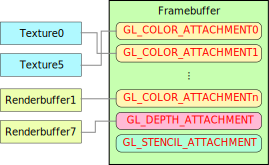
\includegraphics[width=10cm,keepaspectratio]{pics/framebuffer/framebuffer.pdf}
  \end{figure}
\end{frame}


\begin{frame}\frametitle{Usage / Použití FBO}\scriptsize
\begin{enumerate}
  \item Reserve FBO integer id.
  \item Attach textures/renderbuffers
  \item Setup the list of attachments
  \item ...
  \item Bind FBO.
  \item Draw scene.
  \item Unbindg FBO.
  \item Process rendered textures.
\end{enumerate}

\begin{enumerate}
  \item{Získání jména FBO.}
  \item{Připojení textur/renderbufferů k attachmentům.}
  \item{Nastavení seznamu attachmentů.}
  \item{...}
  \item{Aktivování FBO.}
  \item{Vykreslení scény.}
  \item{Deaktivace FBO.}
  \item{Zpracování vyrenderovaných textur.}
\end{enumerate}
\end{frame}

\begin{frame}[fragile]\frametitle{Creation/Deletion / Vytvoření/uvolnění}
  \begin{itemize}
    \item{
    Creation of FVO identifier / Vytvoření FBO identifikátorů:
{\scriptsize
\begin{minted}[bgcolor=bg]{packages/c_cpp.py:CppLexer -x}
void glCreateFramebuffers(GLsizei n,GLuint * buffers);
\end{minted}
}}
    \item{
    Deletion of FBO identifier / Uvolnění FBO identifikátorů:
{\scriptsize
\begin{minted}[bgcolor=bg]{packages/c_cpp.py:CppLexer -x}
void glDeleteFramebuffers(GLsizei n,GLuint * buffers);
\end{minted}
}}
  \end{itemize}
\end{frame}

\begin{frame}[fragile]\frametitle{Check the state / Ověření stavu FBO}\scriptsize
  \begin{itemize}
    \item To check the state of the FBO:
    \item Pro ověření stavu FBO použijeme tuto funkci:
   \end{itemize}

\begin{minted}[bgcolor=bg]{packages/c_cpp.py:CppLexer -x}
GLenum glCheckNamedFramebufferStatus(GLuint fbo,GLenum target);
\end{minted}

  \begin{itemize}
    \item {\color{red} GL\_FRAMEBUFFER\_COMPLETE} -- the state is OK.
    \item Pokud funkce vraci {\color{red} GL\_FRAMEBUFFER\_COMPLETE} je vše v pořádku.
  \end{itemize}
\end{frame}


\begin{frame}[fragile]\frametitle{Bind/Unbind / Aktivování/deaktivování FBO}\scriptsize
\begin{itemize}
  \item To bind/unbind framebuffer:
  \item Aktivování/deaktivování FBO:
\end{itemize}

\begin{minted}[bgcolor=bg]{packages/c_cpp.py:CppLexer -x}
void glBindFramebuffer(GLenum target,GLuint framebuffer);
\end{minted}

\begin{description}
  \item[target] GL\_FRAMEBUFFER $==$ GL\_READ\_FRAMEBUFFER $+$ GL\_DRAW\_FRAMEBUFFER.
  \item[framebuffer] 0 - default framebuffer.
\end{description}
\end{frame}

\begin{frame}[fragile]\frametitle{Attachment of textures / Připojení textur}\scriptsize
\begin{itemize}
  \item One attachment represents one sub buffer of FBO -- for example depth buffer. Attachment of textures:
  \item Attachment představuje jeden podbuffer FBO - například hloubkový buffer.Připojení textur k attachmentům:
\end{itemize}

\begin{minted}[bgcolor=bg]{packages/c_cpp.py:CppLexer -x}
void glNamedFramebufferTexture(GLuint fbo,GLenum attachment,
  GLuint texture,GLint level);
\end{minted}

\begin{description}
\item[fbo] framebuffer
\item[attachment] Attachment type / Které informace budeme zapisovat do textury.
GL\_DEPTH\_ATTACHMENT - depth / hloubkový buffer.
GL\_STENCIL\_ATTACHMENT - stencil / stencil buffer.
GL\_COLOR\_BUFFERx - color, other informations / barva, nebo jiná informace.
    Fragment shader (layout(location=x) / Specifikováno pomocí fragment shaderu (layout).
\item[texture] Texture indentifier. / Identifikátor textury.
\item[level] Mipmap level / Stupeň mipmappingu.

\end{description}

\begin{itemize}
  \item Layered rendering
\end{itemize}

\begin{minted}[bgcolor=bg]{packages/c_cpp.py:CppLexer -x}
void glNamedFramebufferTextureLayer(GLuint fbo,GLenum attachment,
  GLuint texture,GLint level,GLint layer);
\end{minted}

\end{frame}

\begin{frame}[fragile]\frametitle{List of attachments / Seznam attachmentů (MRT)}\scriptsize
\begin{itemize}
  \item List of attachments defines, which color buffer will be rendered.
  \item Nastavením seznamu attachmentů definujeme, do kterých barevných bufferů se bude kreslit.
\end{itemize}

\begin{minted}[bgcolor=bg]{packages/c_cpp.py:CppLexer -x}
void glNamedFramebufferDrawBuffers(GLuint id,GLsizei n,const GLenum * bufs);
\end{minted}

\begin{description}
  \item[id] framebuffer
  \item[n] Nof color buffers / Počet bufferů, do kterých budeme kreslit.
  \item[bufs] Seznam GL\_COLOR\_BUFFERx.
    The index $x$ specifies the location in FS: layout(location=$x$) / Pořadí specifikuje, ke kterému layout ve fragment shaderu bude buffer navázán.
\end{description}
\end{frame}

\begin{frame}[fragile]\frametitle{Full example / Kompletní příklad}\scriptsize
  We want to draw color, normal and depth. Fragment shader:\\
  Do textur budeme vykreslovat barvu, normálu a hloubku. Fragment shader:

\begin{minted}[bgcolor=bg]{packages/graphics.py:GLShaderLexer -x}
#version 430
layout(location=0)out vec4 fragColor;//first output - drawbuffer0
layout(location=1)out vec3 fragNormal;//second output - drawbuffer1
//...
void main(){
  //...
  fragColor=vec4(fCol,1);//color
  fragNormal=(fNor+1)/2;//normal
}
\end{minted}
\end{frame}

\begin{frame}[fragile]\frametitle{Full example / Kompletní příklad}\tiny
    Application -- initialization / Aplikace - inicializace:
\begin{minted}[bgcolor=bg]{packages/c_cpp.py:CppLexer -x}
glTexImage2D(GL_TEXTURE_2D,0,GL_RGBA8F,WIDTH,HEIGHT,0,GL_RGBA,GL_UNSIGNED_BYTE,NULL);//color texture
glTexImage2D(GL_TEXTURE_2D,0,GL_RGB32F,WIDTH,HEIGHT,0,GL_RGBA,GL_UNSIGNED_BYTE,NULL);//normal texture
glTexImage2D(GL_TEXTURE_2D,0,GL_DEPTH_COMPONENT24,WIDTH,HEIGHT,0,GL_DEPTH_COMPONENT,GL_UNSIGNED_BYTE,NULL);//depth texture

glCreateFramebuffers(1,&fbo);//reserve FBO identifier

//attach textures
glNamedFramebufferTexture(fbo,GL_DEPTH_ATTACHMENT,tDepth,0);
glNamedFramebufferTexture(fbo,GL_COLOR_ATTACHMENT3,tColor,0);
glNamedFramebufferTexture(GL_FRAMEBUFFER,GL_COLOR_ATTACHMENT5,tNormal,0);

//setup the list of color attachments
GLenum drawBuffers[]={
  GL_COLOR_ATTACHMENT3,//layout(location=0)out vec4 fragColor;
  GL_COLOR_ATTACHMENT5 //layout(location=1)out vec3 fragNormal;
};
glNamedFramebufferDrawBuffers(fbo,2,drawBuffers);

if(glCheckNamedFramebufferStatus(fbo,GL_FRAMEBUFFER)!=GL_FRAMEBUFFER_COMPLETE)
  std::cerr<<"error\n";
glBindFramebuffer(GL_FRAMEBUFFER,0);
\end{minted}
\end{frame}

\begin{frame}[fragile]\frametitle{Full example / Kompletní příklad}\scriptsize
    Drawing / Kresleni:
\begin{minted}[bgcolor=bg]{packages/c_cpp.py:CppLexer -x}
glBindFramebuffer(GL_FRAMEBUFFER,FBO);//bind framebuffer
glDrawArrays(...);
glBindFramebuffer(GL_FRAMEBUFFER,0);//bind default framebuffer
\end{minted}

\end{frame}

\setbeamercolor{background canvas}{bg=fitblue}
\begin{frame}\frametitle{Hierarchical depth buffer}
\begin{center}
\Huge {\color{white}Hierarchical depth buffer}
\end{center}
\end{frame}
\setbeamercolor{background canvas}{bg=white}

\begin{frame}[fragile]\frametitle{Full example}\tiny
		GLSL - CreateHierarchy:
\begin{minted}[bgcolor=bg]{packages/graphics.py:GLShaderLexer -x}
//vertex shader////////////////////////////////////////////////////////////
#version 430
void main(){
  gl_Position=vec4(0);
}
//geometry shader//////////////////////////////////////////////////////////
#version 430
layout(points)in;
layout(triangle_strip,max_vertices=4)out;
void main(){
  gl_Position=vec4(-1,-1,0,1);EmitVertex();
  gl_Position=vec4(+1,-1,0,1);EmitVertex();
  gl_Position=vec4(-1,+1,0,1);EmitVertex();
  gl_Position=vec4(+1,+1,0,1);EmitVertex();
}
//fragment shader///////////////////////////////////////////////////////////
#version 430
layout(binding=0)uniform sampler2D Last;//last mipmap
layout(location=0)out vec2 fDepth;//output depth
ivec2 Coord=ivec2(gl_FragCoord.xy);//coordinates
void main(void){
  vec2 A=texelFetch(Last,Coord*2+ivec2(0,0),0).xy;
  vec2 B=texelFetch(Last,Coord*2+ivec2(1,0),0).xy;
  vec2 C=texelFetch(Last,Coord*2+ivec2(0,1),0).xy;
  vec2 D=texelFetch(Last,Coord*2+ivec2(1,1),0).xy;
  fDepth=vec2(min(min(A.x,B.x),min(C.x,D.x)),max(max(A.y,B.y),max(C.y,D.y)));
}
\end{minted}
\end{frame}

\begin{frame}[fragile]\frametitle{Kompletní příklad tvorba hier. z-bufferu}\scriptsize
		Initialization / inicializace:
\begin{minted}[bgcolor=bg]{packages/c_cpp.py:CppLexer -x}
glCreateTextures(GL_TEXTURE_2D,1,&Depth);
//texture containing minimal and maximal depth
glBindTexture(GL_TEXTURE_2D,Depth);
glTextureParameteri(Depth,GL_TEXTURE_MAG_FILTER,GL_NEAREST);
glTextureParameteri(Depth,GL_TEXTURE_MIN_FILTER,GL_NEAREST_MIPMAP_NEAREST);
int Size=WSize;
int Level=0;
while(Size>0){//loop over levels
  glTextureImage2DEXT(Depth,GL_TEXTURE_2D,Level++,GL_RG32F,Size,Size,0,GL_RG,
    GL_FLOAT,NULL);//allocate mipmap level
  Size/=2;
}
//render buffer with depth
glCreateRenderbuffers(1,&RBO_Depth);
glNamedRenderbufferStorage(RBO_Depth,GL_DEPTH_COMPONENT,WSize,WSize);

glCreateFramebuffers(1,&FBO);//create FBO identifier
\end{minted}
\end{frame}


\begin{frame}[fragile]\frametitle{Kompletní příklad tvorba hier. z-bufferu}\scriptsize
  Computing hierarchical depth buffer / tvorba hierarchie:
\begin{minted}[bgcolor=bg]{packages/c_cpp.py:CppLexer -x}
glUseProgram(CreateHierarchy);
int Level=1;
int ActSize=WSize/2;
glBindFramebuffer(GL_FRAMEBUFFER,HFBO);//bind framebuffer
glBindTextureUnit(0,Depth);//bind depth texture to tex. unit 0
while(ActSize>0){//while there are
  glViewport(0,0,ActSize,ActSize);//set viewport
  glTextureParameteri(Depth,GL_TEXTURE_BASE_LEVEL,Level-1);//starting mipmap level
  glTextureParameteri(Depth,GL_TEXTURE_MAX_LEVEL,Level-1);//max mipmap level
  glNamedFramebufferTexture(FBO,GL_COLOR_ATTACHMENT0,Depth,Level);
  GLenum DrawBuffers[]={GL_COLOR_ATTACHMENT0};
  glNamedFramebufferDrawBuffers(1,DrawBuffers);
  glDrawArrays(GL_POINTS,0,1);
  Level++;//increment level of mipmap
  ActSize/=2;//actual size of mipmap
}
glBindFramebuffer(GL_FRAMEBUFFER,0);//unbind framebffer
glTextureParameteri(Depth, GL_TEXTURE_BASE_LEVEL, 0);//starting mipmap level
glTextureParameteri(Depth, GL_TEXTURE_MAX_LEVEL, Level-1);//max mipmap level
glViewport(0,0,WSize,WSize);//reset viewport
\end{minted}
\end{frame}


\setbeamercolor{background canvas}{bg=fitblue}
\begin{frame}
\frametitle{Layered Rendering}
\begin{center}
\Huge {\color{white}Layered Rendering}
\end{center}
\end{frame}
\setbeamercolor{background canvas}{bg=white}

\begin{frame}[fragile]
\frametitle{Layered rendering, cube map}
Cube map rendering - CPU
{\scriptsize
\begin{minted}[bgcolor=bg]{packages/c_cpp.py:CppLexer -x}
GLuint cubeMap;
glCreateTextures(GL_TEXTURE_CUBE_MAP,1,&cubeMap);
for(size_t i=0;i<6;++i)
  glTextureImage2DEXT(cubeMap,GL_TEXTURE_CUBE_MAP_POSITIVE_X+i,0,
    GL_RGBA8,width,height,0,GL_RGBA,GL_UNSIGNED_BYTE,nullptr);
//it will attach all six sides of cube map
glNamedFramebufferTexture(cubeMap,GL_COLOR_ATTACHMENT0,cubeMap,0);
\end{minted}
}
\end{frame}

\begin{frame}[fragile]
\frametitle{Layered rendering, cube map}
Cube map rendering - Vertex Shader
{\scriptsize
\begin{minted}[bgcolor=bg]{packages/graphics.py:GLShaderLexer -x}
layout(location=0)in vec3 position;
uniform float near = 0.1;
uniform float far  = 1000;
uniform vec4 lightPosition = vec4(0,0,0,1);
out int vInstanceID;
void main(){
  const mat4 views[6] = {
    mat4(vec4(+0,+0,-1,0), vec4(+0,-1,+0,0), vec4(-1,+0,+0,0), vec4(0,0,0,1)),
    mat4(vec4(+0,+0,+1,0), vec4(+0,-1,+0,0), vec4(+1,+0,+0,0), vec4(0,0,0,1)),
    mat4(vec4(+1,+0,+0,0), vec4(+0,+0,-1,0), vec4(+0,+1,+0,0), vec4(0,0,0,1)),
    mat4(vec4(+1,+0,+0,0), vec4(+0,+0,+1,0), vec4(+0,-1,+0,0), vec4(0,0,0,1)),
    mat4(vec4(+1,+0,+0,0), vec4(+0,-1,+0,0), vec4(+0,+0,-1,0), vec4(0,0,0,1)),
    mat4(vec4(-1,+0,+0,0), vec4(+0,-1,+0,0), vec4(+0,+0,+1,0), vec4(0,0,0,1))
  };

  mat4 projection = mat4(
    vec4(1,0,0,0),
    vec4(0,1,0,0),
    vec4(0,0,-(far+near)/(far-near),-1),
    vec4(0,0,-2*far*near/(far-near),0));
  gl_Position = projection*views[gl_InstanceID]*vec4(position-lightPosition.xyz,1);
  vInstanceID = gl_InstanceID;
}
\end{minted}
}
\end{frame}


\begin{frame}[fragile]
\frametitle{Layered rendering, cube map}
Cube map rendering - Geometry shader
{\scriptsize
\begin{minted}[bgcolor=bg]{packages/graphics.py:GLShaderLexer -x}
layout(triangles)in;
layout(triangle_strip,max_vertices=3)out;
in int vInstanceID[];
void main(){
  gl_Layer = vInstanceID[0];
  gl_Position = gl_in[0].gl_Position;EmitVertex();
  gl_Position = gl_in[1].gl_Position;EmitVertex();
  gl_Position = gl_in[2].gl_Position;EmitVertex();
  EndPrimitive();
}
\end{minted}
}
\end{frame}


